\documentclass[11pt,class=report,crop=false]{standalone}
\usepackage[screen]{../python}

\begin{document}


%====================================================================
\chapitre{Functions}
%====================================================================

\objectifs{Writing a function is the easiest way to group code for a particular task, in order to execute it once or several times later.}


%%%%%%%%%%%%%%%%%%%%%%%%%%%%%%%%%%%%%%%%%%%%%%%%%%%%%%%%%%%%%%%%
%%%%%%%%%%%%%%%%%%%%%%%%%%%%%%%%%%%%%%%%%%%%%%%%%%%%%%%%%%%%%%%%

\begin{cours}[Function (start)]

\index{function}

A computer function is a portion of code that performs a specific task and can be used one or more times during the rest of the program. 
To define a function with \Python{}, it's very simple. 
Here are two examples:
\begin{center}
\begin{minipage}{0.4\textwidth}
\begin{lstlisting}
def say_hello():
    print("Hello world!")
    return
\end{lstlisting}
\end{minipage}\qquad\qquad
\begin{minipage}{0.4\textwidth}
\begin{lstlisting}
def print_squares():
    for i in range(20):
        print(i**2)
    return
\end{lstlisting}
\end{minipage}
\end{center}

\index{def@\ci{def}}

The instructions are grouped into an indented block. The word \ci{return}\index{return@\ci{return}} (optional) indicates the end of the function. These instructions are executed only if I call the function. For example, each time I execute the command \ci{say_hello()}, \Python{} displays the sentence \og{}Hello world!\fg{}. Each time I execute the command \ci{print_squares()}, \Python{} displays $0,1,4,9,16,\ldots$, i.e. the numbers $i^2$ for $i=0,\ldots,19$.

\mybox{
\myfigure{0.7}{
  \tikzinput{fig-functions-lesson-1}
} }


\end{cours}



\begin{cours}[Function (continued)]

Functions achieve their full potential with:
\begin{itemize}
  \item an \defi{input}, which groups variables that serve as \defi{parameters}\index{parameter@parameter}\index{function!parametre@parameter},
  \item an \defi{output}, which is a result returned by the function (and which will often depend on the input parameters).
\end{itemize}

Here are two examples:
\begin{center}
\begin{lstlisting}
def display_month(number):
    if number == 1:
        print("We are in January.")
    if number == 2:
        print("We are in February.")
    if number == 3:
        print("We are in March.")
    # etc.
    return
\end{lstlisting}
\end{center}
When called this function displays the name of the month based on the number provided as input. For example \ci{display_month(3)} will display \ci{"We are in March."}.

\begin{center}
\begin{lstlisting}
def compute_cube(a):
    cube = a * a * a    # or a**3
    return cube
\end{lstlisting}

\end{center}

This function calculates the cube of a number, for example \ci{compute_cube(2)} does not display anything but returns the value \ci{8}. This value can be used elsewhere in the program.
For example, what do the following instructions do?
\begin{center}
\begin{lstlisting}
x = 3
y = 4
z = compute_cube(x) + compute_cube(y)
print(z)
\end{lstlisting}
\end{center}
In mathematical terms, we put $x=3$, $y=4$, then we calculate the cube of $x$, the cube of $y$ and add them up:
$$z = x^3 + y^3 = 3^3 + 4^3 = 27 + 64 = 91$$
Thus the program displays \ci{91}.
\mybox{
\myfigure{0.7}{
  \tikzinput{fig-functions-lesson-2}
} }

The advantages of programming using functions are as follows:
\begin{itemize}
  \item you write the code of a function only once, but you can call the function several times;
  \item by dividing our program into small blocks, each with its own use, the program is easier to write, read, correct and modify;
  \item you can use a function written by someone else (such as the \ci{sqrt()} function) without knowing all the internal details of its programming.
\end{itemize} 

\end{cours}


%%%%%%%%%%%%%%%%%%%%%%%%%%%%%%%%%%%%%%%%%%%%%%%%%%%%%%%%%%%%%%%%
% Activity 1
%%%%%%%%%%%%%%%%%%%%%%%%%%%%%%%%%%%%%%%%%%%%%%%%%%%%%%%%%%%%%%%%

\begin{activite}[First functions]
\objectifs{Goal: write very simple functions.}

\begin{enumerate}
  \item \textbf{Function without parameter or output.}
  \begin{enumerate}
    \item Program a function called \ci{print_table_of_7()} that displays the multiplication table by $7$: $1 \times 7 = 7$, $2\times 7 = 14$\ldots
    
    \item Program a function called \ci{print_hello()} that asks the user for his first name and then displays \og{}Hello\fg{} followed by his name.
    
    \emph{Hint.} Use \ci{input()}.
  \end{enumerate}

  \item \textbf{Function with one parameter and no output.}
  \begin{enumerate}
    \item Program a function called \ci{print_a_table(n)} that depends on a parameter \ci{n} and displays the multiplication table by this integer $n$.
    For example, the command \ci{print_a_table(5)} must display: $1 \times 5 = 5$, $2\times 5 = 10$\ldots
    
    \item Program a function called \ci{say_greeting(sentence)} that depends on a parameter \ci{sentence}. This function asks for the user's first name and displays a greeting followed by the first name. For example, \ci{say_greeting("Hi")} would display \og{}Hi\fg{} followed by the first name given by the user.
  \end{enumerate}  
  
  \item \textbf{Function without parameter and with output.}
  
Program a function called \ci{ask_full_name()} that first asks for the user's first name, then his last name and returns the complete identity with the last name in upper case as a result. For example, if the user enters \og{}Dark\fg{} then \og{}Vador\fg{}, the function returns the string \ci{"Dark VADOR"} (the function displays nothing).

\emph{Hints.} 
\begin{itemize}
  \item If \ci{string} is a string, then \ci{string.upper()}\index{string}\index{upper@\ci{upper}} is the transformed string with characters in capital letters. Example: if \ci{string = "Vador"} then \ci{string.upper()} returns \ci{"VADOR"}.
  
  \item \index{concatenation} You can merge two strings by using the operator \og{}\ci{+}\fg{}. Example: \ci{"Dark" + "Vador"} is equal to \ci{"DarkVador"}.  Another example: if \ci{string1 = "Dark"} and \ci{string2 = "Vador"} then \ci{string1 + " " + string2} is equal to \ci{"Dark Vador"}.
\end{itemize}
\end{enumerate}
\end{activite}


%%%%%%%%%%%%%%%%%%%%%%%%%%%%%%%%%%%%%%%%%%%%%%%%%%%%%%%%%%%%%%%%
%%%%%%%%%%%%%%%%%%%%%%%%%%%%%%%%%%%%%%%%%%%%%%%%%%%%%%%%%%%%%%%%

\begin{cours}[Function (continuation and end for now)]

A function can have several parameters and can return several results.
For example, here is a function that calculates and returns the sum and product of two given input numbers.

\begin{center}
\begin{lstlisting}
def sum_product(a,b):
    """ Computes the sum and product of two numbers. """
    s = a + b
    p = a * b
    return s, p

mysum, myprod = sum_product(6,7)
\end{lstlisting}
\end{center}

The last line calls the function with arguments $6$ (for parameter \ci{a}) and $7$ (for parameter \ci{b}). This function returns two values, the first one is assigned to \ci{mysum} (which is therefore equal to $13$) and the second one to \ci{myprod} (which is equal to $42$).

\mybox{
\myfigure{0.7}{
  \tikzinput{fig-functions-lesson-3}
} }

So let's remember:
\begin{itemize}
  \item There can be several input parameters.
  
  \item There can be several results at the output.
  
  \item Very important! Do not confuse displaying and returning a value.
  The display (by the command \ci{print()}) just displays something on the screen. Most functions do not display anything, but return one (or more) value. This is much more useful because this value can be used elsewhere in the program.
  
  \item As soon as the program encounters the instruction \ci{return}\index{return@\ci{return}}\index{function!return@\ci{return}}, the function stops and returns the result. There may be several times the instruction \ci{return} in a function but only one will be executed. It is also possible not to put an instruction \ci{return} if the function returns nothing.
  
  \item In the instructions of a function, you can of course use other functions!
   
  \item It is important to comment well on your programs. To document a function, you can describe what it does starting with a \emph{docstring}\index{docstring@\emph{docstring}}\index{function!docstring@\emph{docstring}}, i.e. a description (in English) surrounded by three quotation marks:   
  \mycenterline{\ci{""" My function does this and that. """}}
  
  to be placed just after the header.

  
  \item When defining a function, the variables that appear between the parentheses are called the \defi{parameters}; when calling the function, however, the values between the parentheses are called the \defi{arguments}\index{argument}\index{function!argument}. There is of course a correspondence between the two.


\end{itemize}
\end{cours}


%%%%%%%%%%%%%%%%%%%%%%%%%%%%%%%%%%%%%%%%%%%%%%%%%%%%%%%%%%%%%%%%
% Activity 2
%%%%%%%%%%%%%%%%%%%%%%%%%%%%%%%%%%%%%%%%%%%%%%%%%%%%%%%%%%%%%%%%

\begin{activite}[More features]

\objectifs{Goal: build functions with different types of input and output.}

\begin{enumerate}
  \item \textbf{Trinomials.}
  
  \begin{enumerate}
    \item Write a function \ci{trinomial_1(x)} that depends on a parameter \ci{x} and returns the value of the trinomial $3x^2-7x+4$. For example, \ci{trinomial_1(7)} returns \ci{102}.
    
    \item Write a function \ci{trinomial_2(a,b,c,x)} that depends on four parameters \ci{a}, \ci{b}, \ci{c} and \ci{x} and returns the value of the trinomial $ax^2+bx+c$. For example, \ci{trinomial_2(2,-1,0,6)} returns \ci{66}.
  \end{enumerate}   
  
  
  \item \textbf{Currencies.}
  
   \begin{enumerate}
    \item Write a function \ci{conversion_dollars_to_euros(amount)} which depends on a parameter and which for a sum of money \ci{amount}, expressed in dollars, returns its value in euros (you will take for example $1$ dollar = $0.89$ euro).
    
    \item Write a function \ci{conversion_dollars(amount,currency)} which depends on two parameters \ci{amount} and \ci{currency} and converts the amount given in dollars, to the desired currency.
    Examples of currencies: 
    $1$ dollar = $0.89$ euros;
    $1$ dollar = $0.77$ pounds;
    $1$ dollar = $110$ yen.
    For example, \ci{conversion_dollars(100,"pound")} returns $77$.   
    
    
  \emph{Take care to give an intelligible name to your functions and variables. Don't forget to document each function by adding a small explanatory text between triple quotation marks at the very beginning of your function.}
    
    
  \end{enumerate}   
  
  \item \textbf{Volumes.}
  
   Build functions that calculate and return volumes:
  \begin{itemize}
    \item the volume of a cube according to the length of one side,
    \item the volume of a ball according to its radius,
    \item the volume of a cylinder according to the radius of its base and its height,
    \item the volume of a rectangular parallelepiped box according to its three dimensions.
   \end{itemize}
   
   For the value of $\pi$, you will take either the approximate value $3.14$, or the approximate value provided by the constant \ci{pi} of the module \ci{math}.
  
  
  \item \textbf{Perimeters and areas.}
  
  \begin{enumerate}
    \item Write a function whose use is \ci{perimeter_area_rectangle(a,b)} and which returns the perimeter and area of a rectangle with dimensions of $a$ and $b$.
      
    \item Same question with \ci{perimeter_area_disc(r)} for the perimeter and area of a  disc of radius $r$.
    
    \item Use your previous function to guess from which radius, the area of a disc is larger than the perimeter of that disc.
    
    \emph{Hint.} If you want to scan the radius by incrementing the value of $0.1$ each time, you can build a loop as follows:   
    \mycenterline{\ci{for R in range(0,30):}}    
    then make a call to the function by \ci{perimeter_area_disc(R/10)}.
  \end{enumerate}
\end{enumerate}
  

\end{activite}




%%%%%%%%%%%%%%%%%%%%%%%%%%%%%%%%%%%%%%%%%%%%%%%%%%%%%%%%%%%%%%%%
% Activity 3
%%%%%%%%%%%%%%%%%%%%%%%%%%%%%%%%%%%%%%%%%%%%%%%%%%%%%%%%%%%%%%%%

\begin{activite}[Turtle]
\index{turtle}

\objectifs{Goal: define some functions that draw geometric shapes. Creating a function is similar to creating a block with \emph{Scratch}.}

\begin{center}
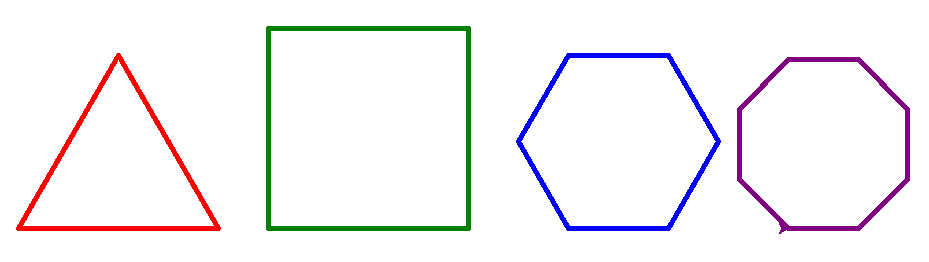
\includegraphics[scale=\myscale,scale=0.4]{screen-functions-tortue}
\end{center}

\begin{enumerate}
  \item Program a function \ci{triangle()} that draws a triangle (in red, each side measuring $200$).

  \item Program a function \ci{square()} that draws a square (in green, each side measuring $200$). Use a loop \og{}for\fg{} so you don't have to rewrite the same instructions several times.  
  
  \item Program a \ci{hexagon(length)} function that draws a hexagon (in blue) of a given side length (the angle to turn is $60$ degrees).
  
  
  \item Program a function \ci{polygon(n,length)} that draws a regular polygon of $n$ sides and a given side length (the angle to rotate is $360/n$ degrees). 
\end{enumerate}

\end{activite}




%%%%%%%%%%%%%%%%%%%%%%%%%%%%%%%%%%%%%%%%%%%%%%%%%%%%%%%%%%%%%%%%
% Activity 4
%%%%%%%%%%%%%%%%%%%%%%%%%%%%%%%%%%%%%%%%%%%%%%%%%%%%%%%%%%%%%%%%

\begin{activite}[Functions again]

\objectifs{Goal: create new functions.}

\begin{enumerate}
  \item 
  
  \begin{enumerate}
  \item 
  Here is the discount for the price of a train ticket based on the age of the passenger:
  \begin{itemize}
    \item reduction of $50\%$ for those under $10$ years old;
    \item reduction of $30\%$ for $10$ to $18$ years old;
    \item reduction of $20\%$ for $60$ years old and over.
  \end{itemize}
  
  Write a function \ci{reduction()} that returns the reduction according to age and whose properties are recalled in the box below:
\begin{fonction}[\ci{reduction()}]
  Use: \ci{reduction(age)} \\
  Input: an integer corresponding to age \\
  Output: an integer corresponding to the reduction
  
  \medskip
    
  Examples: 
  \begin{itemize}
    \item \ci{reduction(17)} returns \ci{30}.
    \item \ci{reduction(23)} returns \ci{0}.
  \end{itemize}
  \end{fonction}  
  
  Deduce a \ci{amount()} function that calculates the amount to be paid based on the normal fare and the traveler's age.
  
\begin{fonction}[\ci{amount()}]
  Use: \ci{amount(normal_rate,age)}\\
  Input: a number \ci{normal_rate} corresponding to the price without discount and \ci{age} (an integer)\\
  Output: a number corresponding to the amount to be paid after reduction\\
  Note: uses the function \ci{reduction()}
  \medskip
    
  Example: \ci{amount(100,17)} returns \ci{70}.
  \end{fonction} 
  
  A family buys tickets for different trips, here is the normal fare for each trip and the ages of the passengers: 
  \begin{itemize}
    \item normal price $30$ dollars, child of $9$ years old;
    
    \item normal price $20$ dollars, for each of the twins of $16$ years old;
    
    \item normal price $35$ dollars, for each parent of $40$ years old.
  \end{itemize}
  What is the total amount paid by the family?
 
  \end{enumerate}
  
  
  \item We want to program a small quiz on the multiplication tables.
  
  \begin{enumerate}
    \item Program a function \ci{is_calculation_correct()} that decides if the answer given to a multiplication is right or not.
    
\begin{fonction}[\ci{is_calculation_correct()}]
  Use: \ci{is_calculation_correct(a,b,answer)} \\
  Input: three integers, \ci{answer} being the proposed answer to the calculation of $a \times b$.\\
  Output: \og{}True\fg{} or \og{}False\fg{}, depending on whether the answer is correct or not
  
  \medskip
    
  Examples: 
  \begin{itemize}
    \item \ci{is_calculation_correct(6,7,35)} returns \ci{False}.
    \item \ci{is_calculation_correct(6,7,42)} returns \ci{True}.
  \end{itemize}
  \end{fonction}  
  
  
    \item Program a function that displays a multiplication, asks for an answer and displays a short concluding sentence. All this in English or a foreign language!
    
\begin{fonction}[\ci{test_multiplication()}]
  Use: \ci{test_multiplication(a,b,lang)} \\
  Input: two integers, the chosen language (for example \ci{"english"} or \ci{"french"})\\
  Output: nothing (but display a sentence)\\
  Note: uses the function \ci{is_calculation_correct()}
  
  \medskip
    
  Example: \ci{test_multiplication(6,7,"french")} asks, in French, for the answer to the calculation $6 \times 7$ and answers if it is correct or not.
  \end{fonction}     
    
  \end{enumerate}
  
  
  \textbf{Bonus.} Improve your program so that the computer offers random operations to the player. (Use the \ci{randint()} function of the module \ci{random}.)
  
\end{enumerate}
\end{activite}




%%%%%%%%%%%%%%%%%%%%%%%%%%%%%%%%%%%%%%%%%%%%%%%%%%%%%%%%%%%%%%%%
% Activity 5
%%%%%%%%%%%%%%%%%%%%%%%%%%%%%%%%%%%%%%%%%%%%%%%%%%%%%%%%%%%%%%%%

\begin{activite}[Experimental equality]

\objectifs{Goal: use the computer to experiment with equality of functions.}

\begin{enumerate}
  \item
  \begin{enumerate}
    \item Build a function \ci{absolute_value(x)} that returns the absolute value of a number (without using the function \ci{abs()} of \Python{}).

    \item Build a function \ci{root_of_square(x)} which corresponds to the calculation of $\sqrt{x^2}$.

  
  \item Two functions (of one variable) $f$ and $g$ are said to be \defi{experimentally equal} if $f(i)=g(i)$ for $i=-100,-99,\ldots,0,1,2,\ldots,100$. Check by computer that the two functions defined by
  $$|x| \qquad \text{ and } \qquad \sqrt{x^2}$$
  are experimentally equal. 
  
  \end{enumerate}
  
  \item
    \begin{enumerate}
    \item Build a two-parameter function \ci{F1(a,b)} that returns $(a+b)^2$. Same thing with \ci{F2(a,b)} that returns $a^2+2ab+b^2$.
 
  \item Two functions of two variables $F$ and $G$ are said to be \defi{experimentally equal} if $F(i,j)=G(i,j)$ for all $i=-100,-99,\ldots,100$ and for all $j = -100,-99,\ldots,100$. Check by computer that the functions defined by $(a+b)^2$ and $a^2+2ab+b^2$ are experimentally equal. 
  
   \item I know that one of the following two identities is true:
   $$(a-b)^3 = a^3 - 3a^2b -3ab^2+b^3 \qquad \text{ or } \qquad (a-b)^3 = a^3 - 3a^2b  + 3ab^2 - b^3.$$
   Help yourself from the computer to decide which one it is!
   
  \end{enumerate} 
  
  \item 
   \begin{enumerate}
    \item Build a function \ci{sincos(x)} that returns $(\sin(x))^2 + (\cos(x))^2$ and another \ci{one(x)} that always returns $1$. Are these two functions experimentally equal (in the sense of the first question)? Find out what could be the cause of this answer.
    
    \item Fix $\epsilon = 0.00001$. It is said that two functions (of one variable) $f$ and $g$ are \defi{experimentally approximately equal} if $|f(i)-g(i)| \le \epsilon$ for $i=-100,-99,\ldots,100$. Do the two functions defined by \ci{sincos(x)} and \ci{one(x)} now check this criterion?
    
    \item Experimentally check and experimentally approximately check the identities:
    $$\sin(2x) = 2\sin(x)\cos(x), \qquad \cos\left(\frac\pi2-x\right)=\sin(x).$$

  
  \item \textbf{Bonus. A counter-example.}
  Show that the functions defined by $g_1(x) = \sin(\pi x)$ and $g_2(x)=0$ are experimentally equal (with our definition given above). But also show that you don't get $g_1(x) = g_2(x)$ for every $x\in\Rr$.
  
  \end{enumerate} 
\end{enumerate}

\end{activite}


\begin{cours}[Local variable]


Here is a very simple function that takes a number as an input and returns the number increased by one.
\begin{center}
\begin{lstlisting}
def my_function(x):
    x = x + 1
    return x
\end{lstlisting}
\end{center}

\begin{itemize}
  \item Of course \ci{my_function(3)} returns \ci{4}.
  
  \item If I define a variable by \ci{y = 5} then \ci{my_function(y)} returns \ci{6}. And the value of \ci{y} has not changed, it is still equal to \ci{5}.
  
  \item Here is the delicate situation that you must understand:
\begin{center}
\begin{lstlisting}
x = 7
print(my_function(x))
print(x)
\end{lstlisting}
\end{center}
  \begin{itemize}
    \item The variable \ci{x} is initialized to \ci{7}.
    
    \item The call of the function \ci{my_function(x)} is therefore the same as 
     \ci{my_function(7)} and logically returns \ci{8}.
     
    
    \item What is the value of \ci{x} at the end? The variable \ci{x} is unchanged and is still equal to \ci{7}! Even if in the meantime there has been an instruction \ci{x = x + 1}. This instruction changed the \ci{x} inside the function, but not the \ci{x} outside the function.
\end{itemize}   
\end{itemize} 
 
\bigskip

\begin{itemize}
  \item Variables defined within a function are called 
\defi{local variables}\index{local variable}. 
They do not exist outside the function.
  
  \item If there is a variable in a function that has the same name as a variable in the program (like the \ci{x} in the example above), it is as if there were two distinct variables; the local variable only exists inside the function.
  
\end{itemize}


To understand the scope of the variables, you can color the global variables of a function in red, and the local variables with one color per function.
The following small program defines a function that adds one and another that calculates the double.

\mybox{
\myfigure{0.7}{
  \tikzinput{fig-functions-lesson-4}
} }

The program first displays the value of \ci{x}, so \ci{7}, then it increases it by $1$, so it displays \ci{8}, then it displays twice as much as \ci{x}, so \ci{14}. The global variable \ci{x} has never changed, so the last display of \ci{x} is still \ci{7}.

\bigskip

It is still possible to force the hand to \Python{} and modify a global variable in a function using the keyword \ci{global}. See the chapter \og{}Polish calculator -- Stacks\fg{}.

\end{cours}

\end{document}
